\documentclass[tikz, border={5mm 5mm 5mm 5mm}]{standalone}

\usepackage[sfdefault]{FiraSans}
\usetikzlibrary{positioning}
\usetikzlibrary{quotes}
\usetikzlibrary{shapes.misc}
\usetikzlibrary{arrows.meta}
\usetikzlibrary{calc}

\newcommand*\circled[1]{\tikz[baseline= (char.base)]{%
    \node[shape=circle, draw, inner sep=2pt] (char) {#1};}}

\tikzset{%
    repo/.style={%
        draw,
        minimum width=25mm,
        minimum height=10ex,
        rounded corners,
        align=center,
        very thick,
    },
    origrepo/.style={%
        repo,
        draw=green!70!black,
    },
    gitservice/.style={%
        draw=red!50,
        very thick,
        rounded corners,
        minimum width=30mm,
        minimum height=30mm,
        text depth=19mm,
    },
    prstep/.style={%
        font={\small},
        align=center,
        midway,
    },
    origarrow/.style={%
        >={Stealth[round]},
        thick,
        draw=green!80,
    },
}

\begin{document}

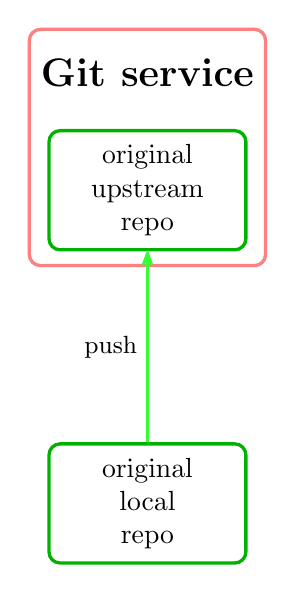
\begin{tikzpicture}
    \node[gitservice] (gitservice) {\Large \textbf{Git service}};

    \node[origrepo, anchor=south]
        (ownerupstream) at ($(gitservice.south) + (0, 0.2)$)
        {original\\upstream\\repo};

    \node[origrepo]
        (ownerlocal) at ($(gitservice.south) - (0, 3)$)
        {original\\local\\repo};

    \draw[origarrow, ->]
        (ownerlocal.north) -- (ownerupstream.south)
        node[prstep, left] {push};
\end{tikzpicture}

\end{document}
